\chapter{Fundamentals} % and theoretical background (BASICS)
\label{ch:fundamentals}

\section{Surface representations}
\label{sec:surface_representations}

CAD and CAM software use several different representations for final and intermediate geometric parts like cutter geometries, the manufactured work piece or the current machining state.
Tukora provides a comprehensive list with sketches and descriptions of the most commonly used representations \cite{virtual_machining_review}. These will be discussed in this section. 

\begin{description}
	\item[Vector clipping] \hfill \\
	Vector clipping is mainly used in CAE to verify the correctness of a generated (C)NC program before it is run on an actual milling machine and has been first described by Chappel \cite{vector_clipping}.
	The method requires the geometries of the final work piece as well as the stock (\ie the original piece of material it has been cut out of).
	Initially, points on the final work piece are calculated together with surface normals (\ie a point cloud) where the normals are not necessary of unit length but long enough to reach the surface of the stock.
	To simulate the manufacturing process, the cutter is moved over this point cloud and the vectors attached to the points are clipped by the moving cutter (\cf figure \ref{fig:vector_clipping}).
	Tukora compares this method to a lawn mower, which cuts the grass (\ie the normal vectors) towards the ground (\ie the final work piece).
	After cutting has completed, the lengths of the remaining vectors indicate the local error of the (C)NC program.
	Vectors with positive lengths mark areas where too less material has removed and vice versa.
	The vector lengths are finally used to color the final work piece where the color indicates the severity of the machining error. 
	
	\begin{figure}[h]
		\centering
		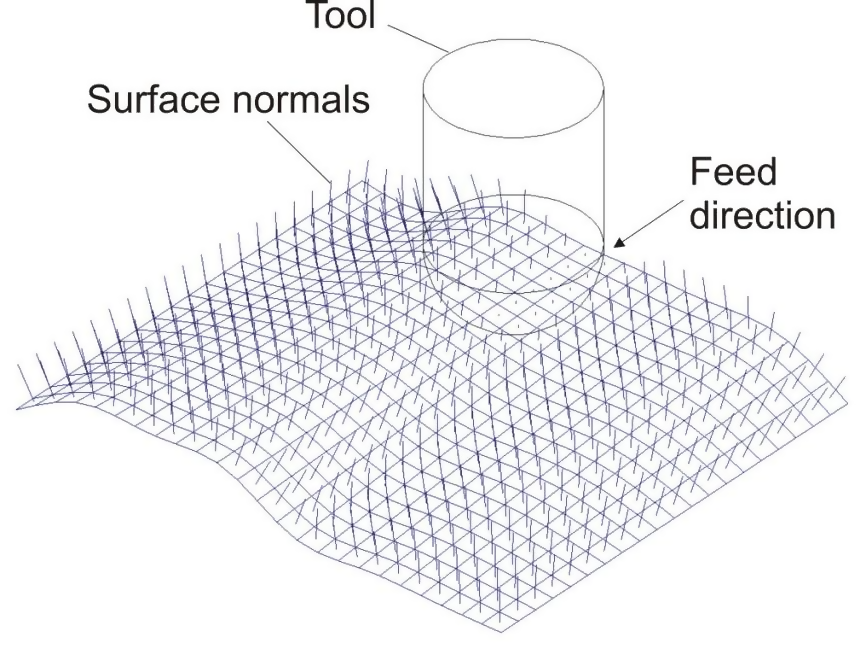
\includegraphics[width=0.5\textwidth]{images/vector_clipping}
		\caption{The vector clipping method as described by Chappel \cite{vector_clipping}. Image by Tukora \cite{virtual_machining_review}.}
		\label{fig:vector_clipping}
	\end{figure}
	 
	\item[Z-maps and depth images] \hfill \\
	Describing geometries using z-maps has been first described by Anderson \cite{zmap}.
	
	\begin{figure}[h]
		\centering
		\begin{subfigure}[b]{0.4\textwidth}
			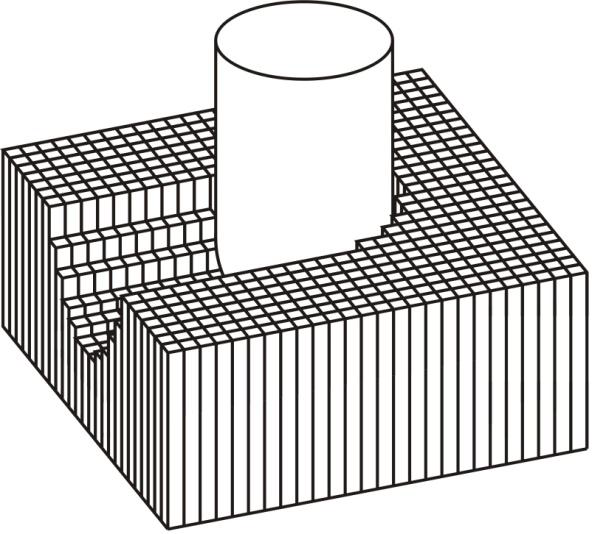
\includegraphics[width=\textwidth]{images/zmap}
			\caption{z-map}
		\end{subfigure}
		\begin{subfigure}[b]{0.4\textwidth}
			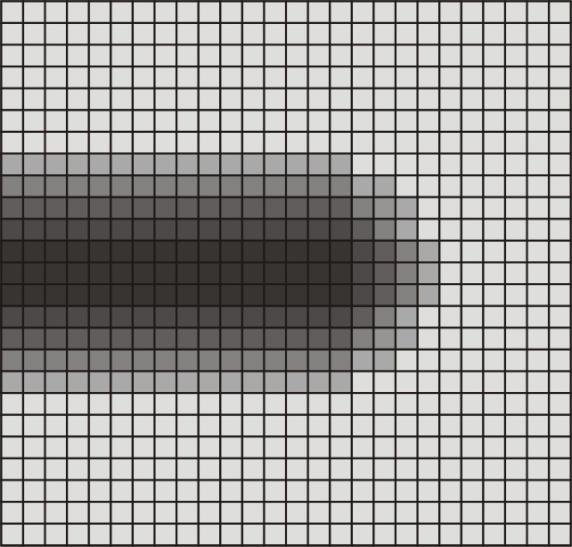
\includegraphics[width=\textwidth]{images/depth_image}
			\caption{depth image}
		\end{subfigure}
		\caption{aa}
		\label{fig:zmap_depth_image}
	\end{figure}
	
	\item[Dexel images]
	
	\item[Multi-dexel images]
	
	\item[Constructive Solid Geometry (CSG)]
	
	\item[Uniform spacial decomposition (USD)]
	
	\item[Hierarchical spacial decomposition (HSD)]
	
	\item[Boundary representation (BRep)]
	
\end{description}

Implicit models may be composed of polygons, parametric surfaces and functional representations (iso surfaces).

Furthermore, many and also different types of such surfaces may be aggregated, referred to as B-rep (boundary representation), or combined using set operations such as in CSG.



\section{Triangulations}
\label{sec:definitions}

\begin{description}
	\item[Triangulation/Tesselation]
	
	\item[Mesh]
	
	\item[Manifold]
	
	\item[Oriented]
	
	\item[Closed/water-tight]
	
	\item[Boundary]
	
	\item[Voronoi]
	
	\item[Delaunay]
	A triangulation is called Delaunay when the circumcircle of each triangle does not contain a vertex of another triangle.
	Delaunay triangulations produce very regular and visually appealing triangle meshes.
	
	\item[Gabriel 2-Simplex]
	
	\item[Chord error]
	
\end{description}


\section{Surface reconstruction}
\label{sec:surface_reconstruction}

where is surface reconstruction used?
